%!TEX root = ..\Main.tex
\section{Results}
The mean length of each test, excluding the two first tasks used for training, were $11.8$ minutes, with a standard
deviation of $4.4$ minutes - the longest being $28.3$ minutes and the shortest $5.8$ minutes.

Our system produces on average $17$ events from test participants, within which our setup is expected to predict
usability problems, and standard deviation of $4$. One participant produced the most with $26$ and the least produced
was $11$,

The ratio between area designated to containing UPs, referred to as events, and areas that do not contain UPs, in on
average $0.39$, i.e. a little more than 60\% of the data on which we attempt to predict UPs is \textit{normal} data. The
implication of this is that if a classifier were to distribute random guesses based on our data, about 60\% of them
would fall within normal data, and 40\% within data that contains UPs, slightly shifting the difficulty to our
disadvantage. The standard deviation in this ratio is $0.06$, and in only one case, is the area containing UPs larger
with a ration of $0.58$. The smallest example showed $0.25$, i.e. 25\%, of the test consisting of events containing
usability problems.

\newcommand{\fuckinggraph}[4]{
    \begin{figure}[h!]
    \begin{minipage}[t]{0.5\textwidth}
        \includegraphics[width=\linewidth,keepaspectratio=true]{graphics/graphs/#1/#2}
        \caption{#3}
        \label{#4}
    \end{minipage}
    \end{figure}
}

\newcommand{\fuckinggraphevenidontwanttorepeatmyself}[4]{ %short sensor caption1 label1
  \fuckinggraph{#1}
  {False_cover_rate_(FCR)-Events_hit_rate_(EHR)-CovNu-#2.pdf}{#3}{#4}
  %{False_cover_rate_(FCR)-Precision-CovNu-#2.pdf}{#5}{#6}
}

\fuckinggraphevenidontwanttorepeatmyself{short}{GSR}
{GSR showing events hit percent and unwanted area covered. Nu value shade: 0 = green, 1 = red}{fig:gsr_event_ehr}
%{GSR showing precision and unwanted area covered}         {lab:gsr_pres_ehr}

\fuckinggraphevenidontwanttorepeatmyself{short}{EEG}
{EEG showing events hit percent and unwanted area covered. Nu value shade: 0 = green, 1 = red}{fig:eeg_event_ehr}
%{EEG showing precision and unwanted area covered}         {lab:eeg_pres_ehr}

\fuckinggraphevenidontwanttorepeatmyself{short}{HR}
{Heart rate showing events hit percent and unwanted area covered. Nu value shade: 0 = green, 1 = red}{fig:hr_event_ehr}
%{Heart rate showing precision and unwanted area covered}         {fig:hr_pres_ehr}

\fuckinggraphevenidontwanttorepeatmyself{short}{FACE}
{Kinect showing events hit percent and unwanted area covered. Nu value shade: 0 = green, 1 = red}{fig:face_event_ehr}
%{Kinect showing precision and unwanted area covered}         {lab:face_pres_ehr}

Having performed a grid search to find optimal settings for our one-class SVM classification, we performed the mentioned
Nu-value line search. Figures~\ref{fig:gsr_event_ehr},\ref{fig:hr_event_ehr} and \ref{fig:face_event_ehr}
shows the result of this as scatter plots of EHR and FCR for each sensor. Nu values range from low/green to high/red,
ranging from $0.01$ to $1.00$ in $0.01$ intervals, yielding 100 different settings and results for each test
participant. All test participants are represented in each graph, and Nu-values with a thick border is the average of
each Nu-value across all test participants.

\paragraph{Sensors likeness and differences}
Looking at Figures~\ref{fig:gsr_event_ehr}, \ref{fig:eeg_event_ehr}, \ref{fig:hr_event_ehr} and \ref{fig:face_event_ehr},
as well as Table~\ref{[TABLE]_avg_stats_sensors}, it can be seen that choosing a higher Nu-value for your classifier can yield interesting propositions if the classifier should cover as many problems as possible while minimizing the area wrongly covered.
\begin{table}[H]
  \centering
  \textbf{GSR}\vspace{2pt}
  \begin{tabularx}{\columnwidth}{cXXc}
    \toprule
    \textbf{Nu} & \textbf{Precision} & \textbf{EHR} & \textbf{FCR} \\
    \midrule
    1.0\% & 30.0\% & 4.5\% & 2.1\% \\ \hline
    5.0\% & 36.4\% & 14.5\% & 7.2\% \\ \hline
    25.0\% & 39.0\% & 36.6\% & 23.5\% \\ \hline
    50.0\% & 37.8\% & 63.0\% & 44.8\% \\ \hline
    75.0\% & 37.6\% & 84.0\% & 70.6\% \\ \hline
    100.0\% & 37.1\% & 99.8\% & 99.8\% \\ \hline
    \bottomrule
  \end{tabularx}

  \vspace{4pt}

  \textbf{EEG}\vspace{2pt}
  \begin{tabularx}{\columnwidth}{cXXc}
    \toprule
    \textbf{Nu} & \textbf{Precision} & \textbf{EHR} & \textbf{FCR} \\
    \midrule
    1.0\% & 43.7\% & 23.8\% & 18.5\% \\ \hline
    5.0\% & 38.6\% & 35.1\% & 20.9\% \\ \hline
    25.0\% & 35.0\% & 68.5\% & 61.8\% \\ \hline
    50.0\% & 36.7\% & 90.3\% & 86.1\% \\ \hline
    75.0\% & 37.0\% & 91.7\% & 90.8\% \\ \hline
    100.0\% & 37.2\% & 93.7\% & 95.8\% \\ \hline
    \bottomrule
  \end{tabularx}

  \vspace{4pt}

  \textbf{Kinect}\vspace{2pt}
  \begin{tabularx}{\columnwidth}{cXXc}
    \toprule
    \textbf{Nu} & \textbf{Precision} & \textbf{EHR} & \textbf{FCR} \\
    \midrule
    1.0\% & 51.7\% & 21.7\% & 10.0\% \\ \hline
    5.0\% & 50.8\% & 33.1\% & 28.5\% \\ \hline
    25.0\% & 44.1\% & 64.8\% & 57.4\% \\ \hline
    50.0\% & 40.5\% & 89.0\% & 75.7\% \\ \hline
    75.0\% & 37.5\% & 98.2\% & 92.5\% \\ \hline
    100.0\% & 36.5\% & 99.6\% & 96.2\% \\ \hline
    \bottomrule
  \end{tabularx}

  \vspace{4pt}

  \textbf{Heart rate}\vspace{2pt}
  \begin{tabularx}{\columnwidth}{cXXc}
    \toprule
    \textbf{Nu} & \textbf{Precision} & \textbf{EHR} & \textbf{FCR} \\
    \midrule
    1.0\% & 31.4\% & 10.1\% & 4.3\% \\ \hline
    5.0\% & 36.0\% & 28.5\% & 15.1\% \\ \hline
    25.0\% & 36.4\% & 61.5\% & 45.5\% \\ \hline
    50.0\% & 35.6\% & 87.1\% & 67.2\% \\ \hline
    75.0\% & 36.1\% & 96.8\% & 86.1\% \\ \hline
    100.0\% & 36.7\% & 99.8\% & 99.3\% \\ \hline
    \bottomrule
  \end{tabularx}

  \caption{Average statistics for each sensor}
  \label{[TABLE] avg_stats_sensors}
\end{table}
In other words if one's aim is to hit all events, a high Nu-value must be chosen, but comes with the trade-off of placing more anomalies outside events. 
While the GSR and the HR both have a smooth curve through the averages of which indicates a stable classifier, but the Kinect seem to be more unstable in its relation between EHR and FCR. However Kinect seems to regain some of its stability with higher Nu values. As shown in \ref{[TABLE]_avg_stats_sensors} and seen in Figure~\ref{fig:eeg_event_ehr}, the EEG deviate from the other sensor by already at low Nu-values doing a very aggressive prediction approach and creating useless predictions at Nu-values above 0.5.

All the graph reveals that across all the test participants no golden Nu-value presents itself. A conservative
setting could be chosen, to ensure that little false area is covered, while still detecting some usability problems. On
the other hand, a higher and more ``aggressive'' value could be chosen in attempt to detect as many problems as
possible, with the trade-off of alse receiving many false-positives. Figures~\ref{fig:gsr_event_ehr},
\ref{fig:eeg_event_ehr}, \ref{fig:hr_event_ehr} and \ref{fig:face_event_ehr} and Table~\ref{[TABLE]_avg_stats_sensors}
shows that the HR, Kinect and GSR manages to have a reasonable across EHR given the FCR the different Nu values, which shows a robustness to the result.

\paragraph{Investigating the best results}
We find it interesting to consider the best performing test participants to see if there difference to be found between them and the rest of the test set. 
If such differences are found, it would be valuable information for future studies because a preliminary screening could help select the people who would fit the research the best.
Figure~\ref{fig:best_five_gsr}. and Tabel~\ref{tab:best_five_avg_stats} shows average statistics for both the five best, and
the best performing across all test participants on the GSR sensor. 
The best are calculated from the sum of EHR for all of the Nu-values to a given test participant.
\newcommand{\graphtheshit}[3]{
    \begin{figure}[h!]
    \begin{minipage}[t]{0.5\textwidth}
        \includegraphics[width=\linewidth,keepaspectratio=true]{graphics/graphs/best-worst/#1}
        \caption{#2}
        \label{#3}
    \end{minipage}
    \end{figure}
}

\newcommand{\somethingsomething}{
  \graphtheshit{best-False_cover_rate_(FCR)-Events_hit_rate_(EHR)-CovNu-GSR.pdf}
  {Five best performing test participants using GSR as sensor. Nu value shade: 0 = green, 1 = red}{fig:best_five_gsr}
}

\somethingsomething
\begin{table}[h]
  \centering
  \textbf{Avegrage for GSR for five best performing}\vspace{2pt}
  \begin{tabularx}{\columnwidth}{cXXc}
    \toprule
    \textbf{Nu} & \textbf{Precision} & \textbf{EHR} & \textbf{FCR} \\
    \midrule
    0.01        & 38.8\%             & 6.4\%        & 3.0\%        \\ \hline
    0.05        & 29.4\%             & 24.6\%       & 9.0\%        \\ \hline
    0.25        & 35.4\%             & 66.5\%       & 30.0\%       \\ \hline
    0.50        & 37.3\%             & 87.6\%       & 53.5\%       \\ \hline
    0.75        & 38.8\%             & 98.7\%       & 75.1\%       \\ \hline
    1.00        & 38.6\%             & 100.0\%      & 100.0\%      \\ \hline
    \bottomrule
  \end{tabularx}

  \textbf{GSR for best performing}\vspace{2pt}
  \begin{tabularx}{\columnwidth}{cXXc}
    \toprule
    \textbf{Nu} & \textbf{Precision} & \textbf{EHR} & \textbf{FCR} \\
    \midrule
    0.01        & 37.9\%             & 7.7\%        & 1.1\%        \\ \hline
    0.05        & 33.5\%             & 30.8\%       & 4.3\%        \\ \hline
    0.25        & 22.8\%             & 76.9\%       & 25.3\%       \\ \hline
    0.50        & 21.3\%             & 92.3\%       & 37.7\%       \\ \hline
    0.75        & 25.5\%             & 100.0\%      & 51.2\%       \\ \hline
    1.00        & 26.2\%             & 100.0\%      & 100.0\%      \\ \hline
    \bottomrule
  \end{tabularx}
  \caption{Average stats for top five, and top performing test participants on GSR}
  \label{tab:best_five_avg_stats}
\end{table}
A noticeable difference for the five best scoring test subjects is their average from the introvert/extrovert Big5 group, which is on average 25.4, SD 2.2.
The total average is 29.49 which is higher than the average for the best five, however the standard deviation is 7.96 which is a quite high fluctuation. 
This is an interesting result because as mentioned in \cite{extrovsintro}, the introvert has shown more ``peaky traces'' when measuring GSR data.
However, since it is only the five best nothing conclusive can be said. 
It could be an interesting topic for further investigation.\\\\
Figure~\ref{[Fig] best result} depicts a test with the points of interest created by the GSR from the best test participant, according to EHR.
Even though the test participant achieved an EHR at 92.3\%  while only having a FCR at 37.7\%. However looking at Figure~\ref{[Fig] best result} the points of interest seems more arbitrary than definitive detection of usability problems.
    \begin{figure}[H]
    \begin{minipage}[t]{0.5\textwidth}
        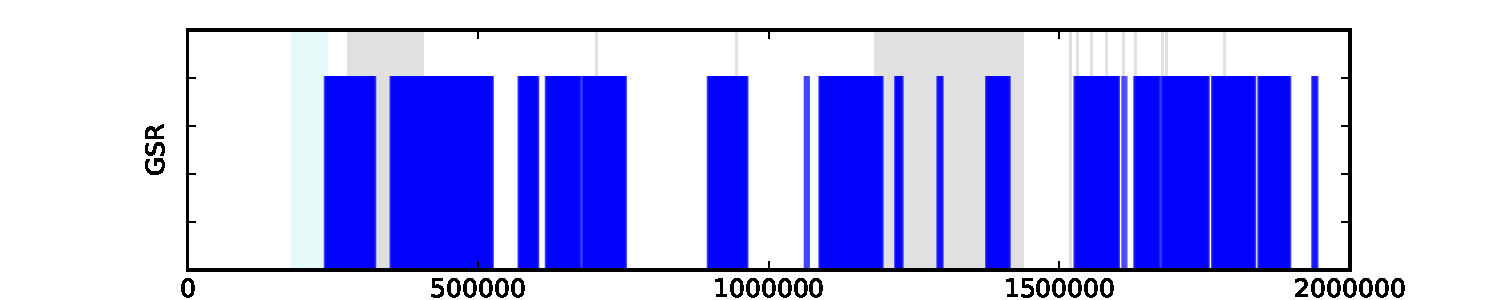
\includegraphics[width=\linewidth,keepaspectratio=true]{graphics/graphs/events/johnny-nu050-29-short-sensors.pdf}
        \caption{Figure showing the detected points of interest(blue) by the GSR from the best test participant at Nu value 0.5. The green area represent the two first task and the grey line and areas represent the events.}
        \label{[Fig] best result}
    \end{minipage}
    \end{figure}
